\chapter{Characterization of $\thetath$}
\label{ch:appendix_b}

In this chapter, a brief analysis of the threshold $\thetath$ is
offered in order to show its dependence on some of the scenario parameters, for
instance:

\begin{itemize}
    \item Number of antennas of the \gls{mimo} configuration.
    \item \gls{snr} of the system.
    \item Cluster size.
    \item Path loss exponent $\gamma$.
\end{itemize}

Figures \ref{fig:th_exp_tiers} through \ref{fig:th_snr_ant} show this dependence
for a series of combinations of parameters.

First, \reff{fig:th_snr_tiers} and \reff{fig:th_snr_ant} show how the threshold
is consistently independent from the \gls{snr}, except for very low values of
it.

For increasing values of the path loss exponent, the threshold increases as
well, as it can be seen in \reff{fig:th_exp_tiers} and \reff{fig:th_exp_ant}. A
higher path loss exponent translates into a lower level of interference between
adjacent cells, in which case coordination may not help at all, so each \gls{bs}
better serves its own users independently. This is the reason for a higher
threshold, which implies that less users will select \gls{bd} as their preferred
transmission strategy.

Another interesting characteristic that is clear in \reff{fig:th_exp_ant} and
\reff{fig:th_snr_ant} is how the number of antennas plays no role in the
threshold.

These two suggestions mean the advantages that \gls{mimo} has to offer have
no influence on the value of the $\thetath$, and it should depend mainly on the
propagation characteristics of the channel.

This claim can be supported by \reff{fig:th_exp_tiers} and
\reff{fig:th_snr_tiers}, which show the behavior of the threshold with the
cluster size, and by the already mentioned dependence on the path loss exponent.
Cluster size is represented by the number of hexagonal tiers that form the
cluster, so that 1 tiers is a 7 cells cluster, 2 tiers is a 19 cells cluster,
and 3 tiers corresponds to a 37 cells cluster.

Similarly to what happened with the path loss exponent, a bigger cluster means
that cells within a cluster may be too far away from some users in the cluster,
who may not benefit much from coordination. As observed with the path loss
exponent $\gamma$, reducing the level of influence among the cells in the
cluster increases the value of the threshold, in this case when the cluster
considered grows in size. Again, this higher value of $\thetath$ means that more
users will select \gls{su} as their transmission strategy.

\begin{figure}[t]
	\centering
	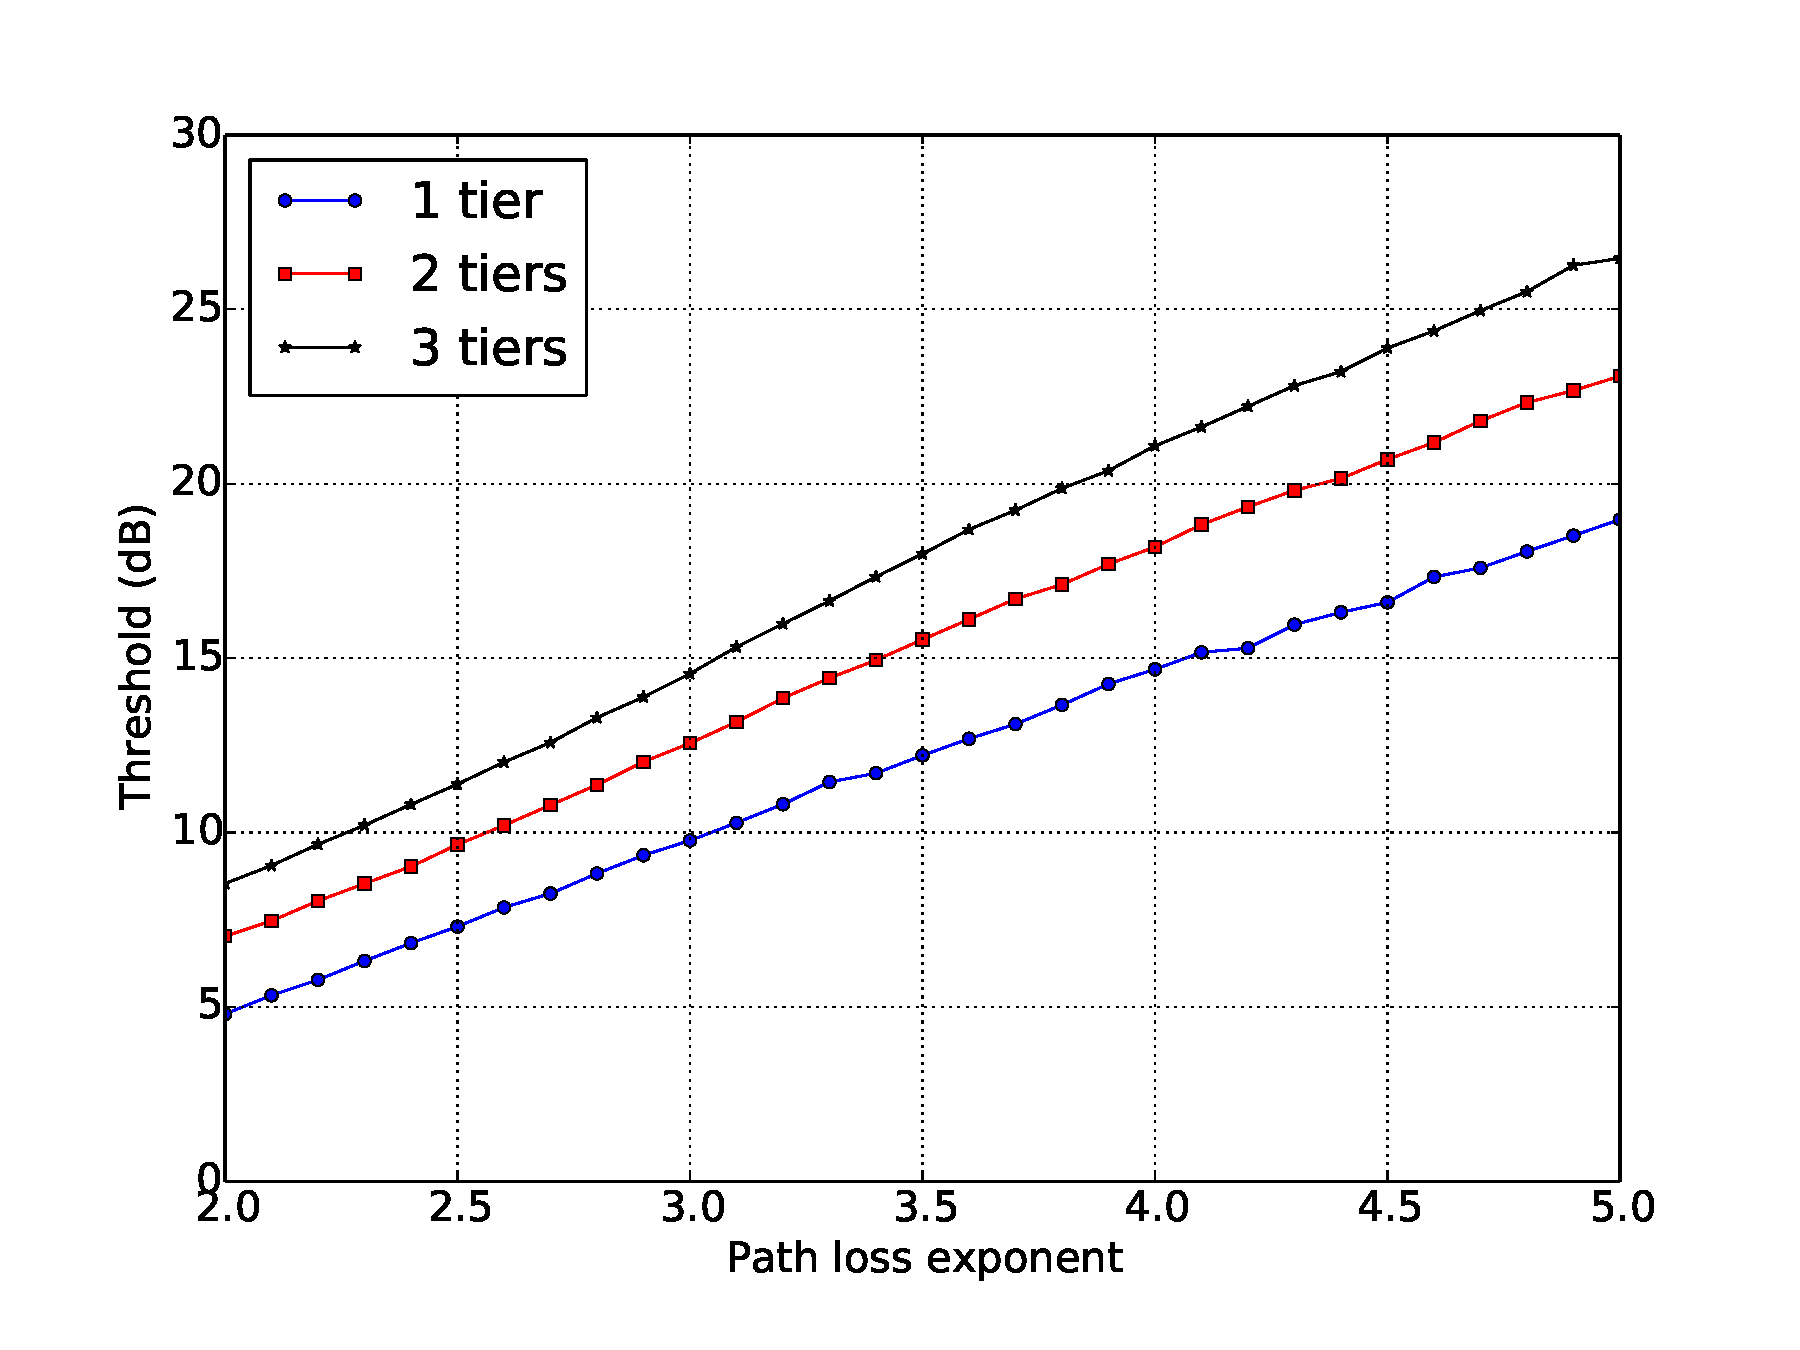
\includegraphics[width=0.75\columnwidth]{./21.appendices/figure/threshold_exp_tiers_02x02_s+0015_r1300}
	\caption{Threshold as a function of the path loss exponent, for different
    cluster sizes, for an \gls{snr} of $15$\,dB.}
	\label{fig:th_exp_tiers}
\end{figure}

\begin{figure}[t]
	\centering
	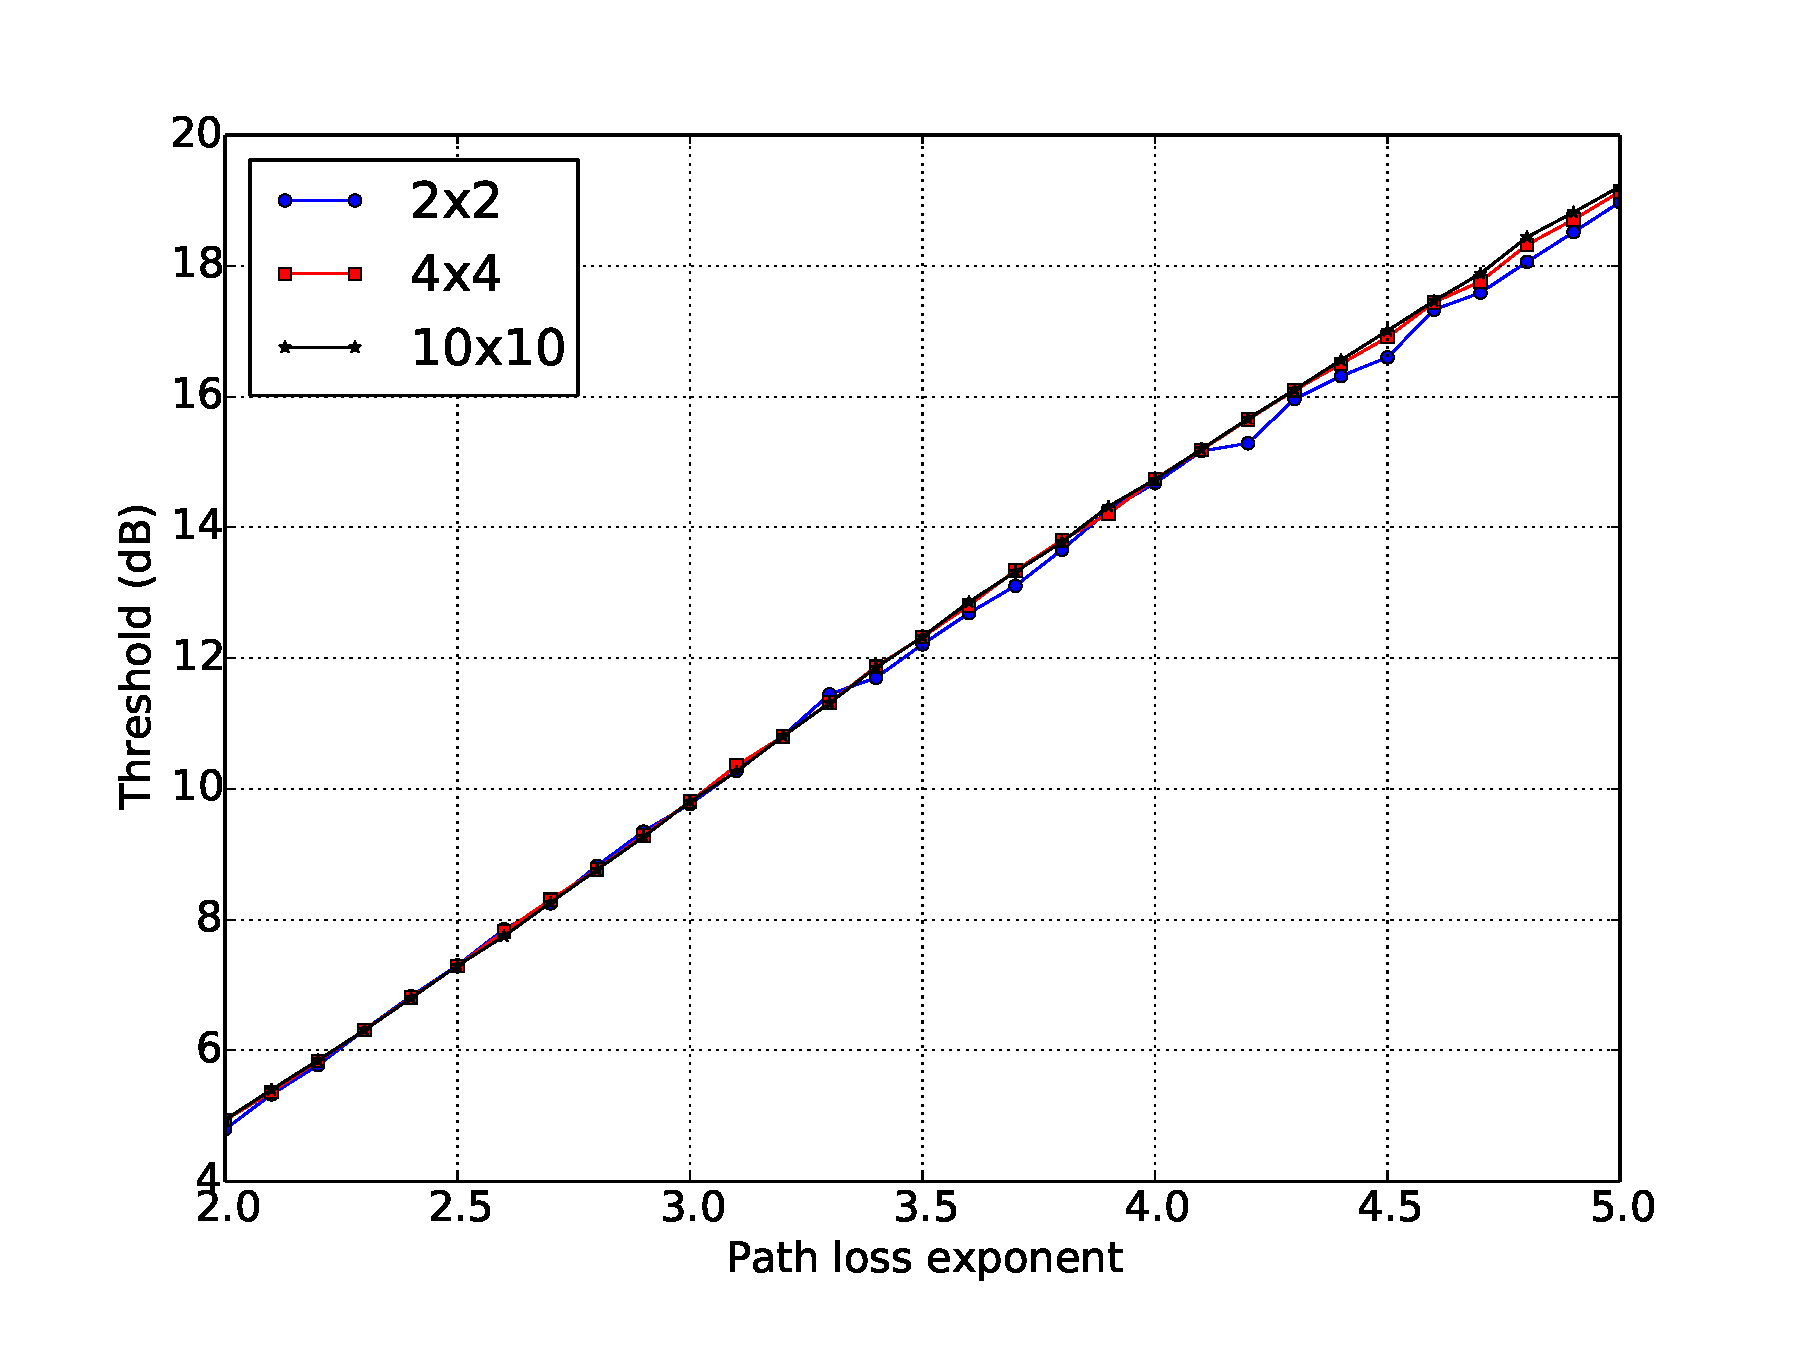
\includegraphics[width=0.75\columnwidth]{./21.appendices/figure/threshold_exp_anten_02x02_t02_i01_r1300}
	\caption{Threshold as a function of the path loss exponent, for different
    \gls{mimo} configurations, for an \gls{snr} of $15$\,dB.}
	\label{fig:th_exp_ant}
\end{figure}

\begin{figure}[t]
	\centering
	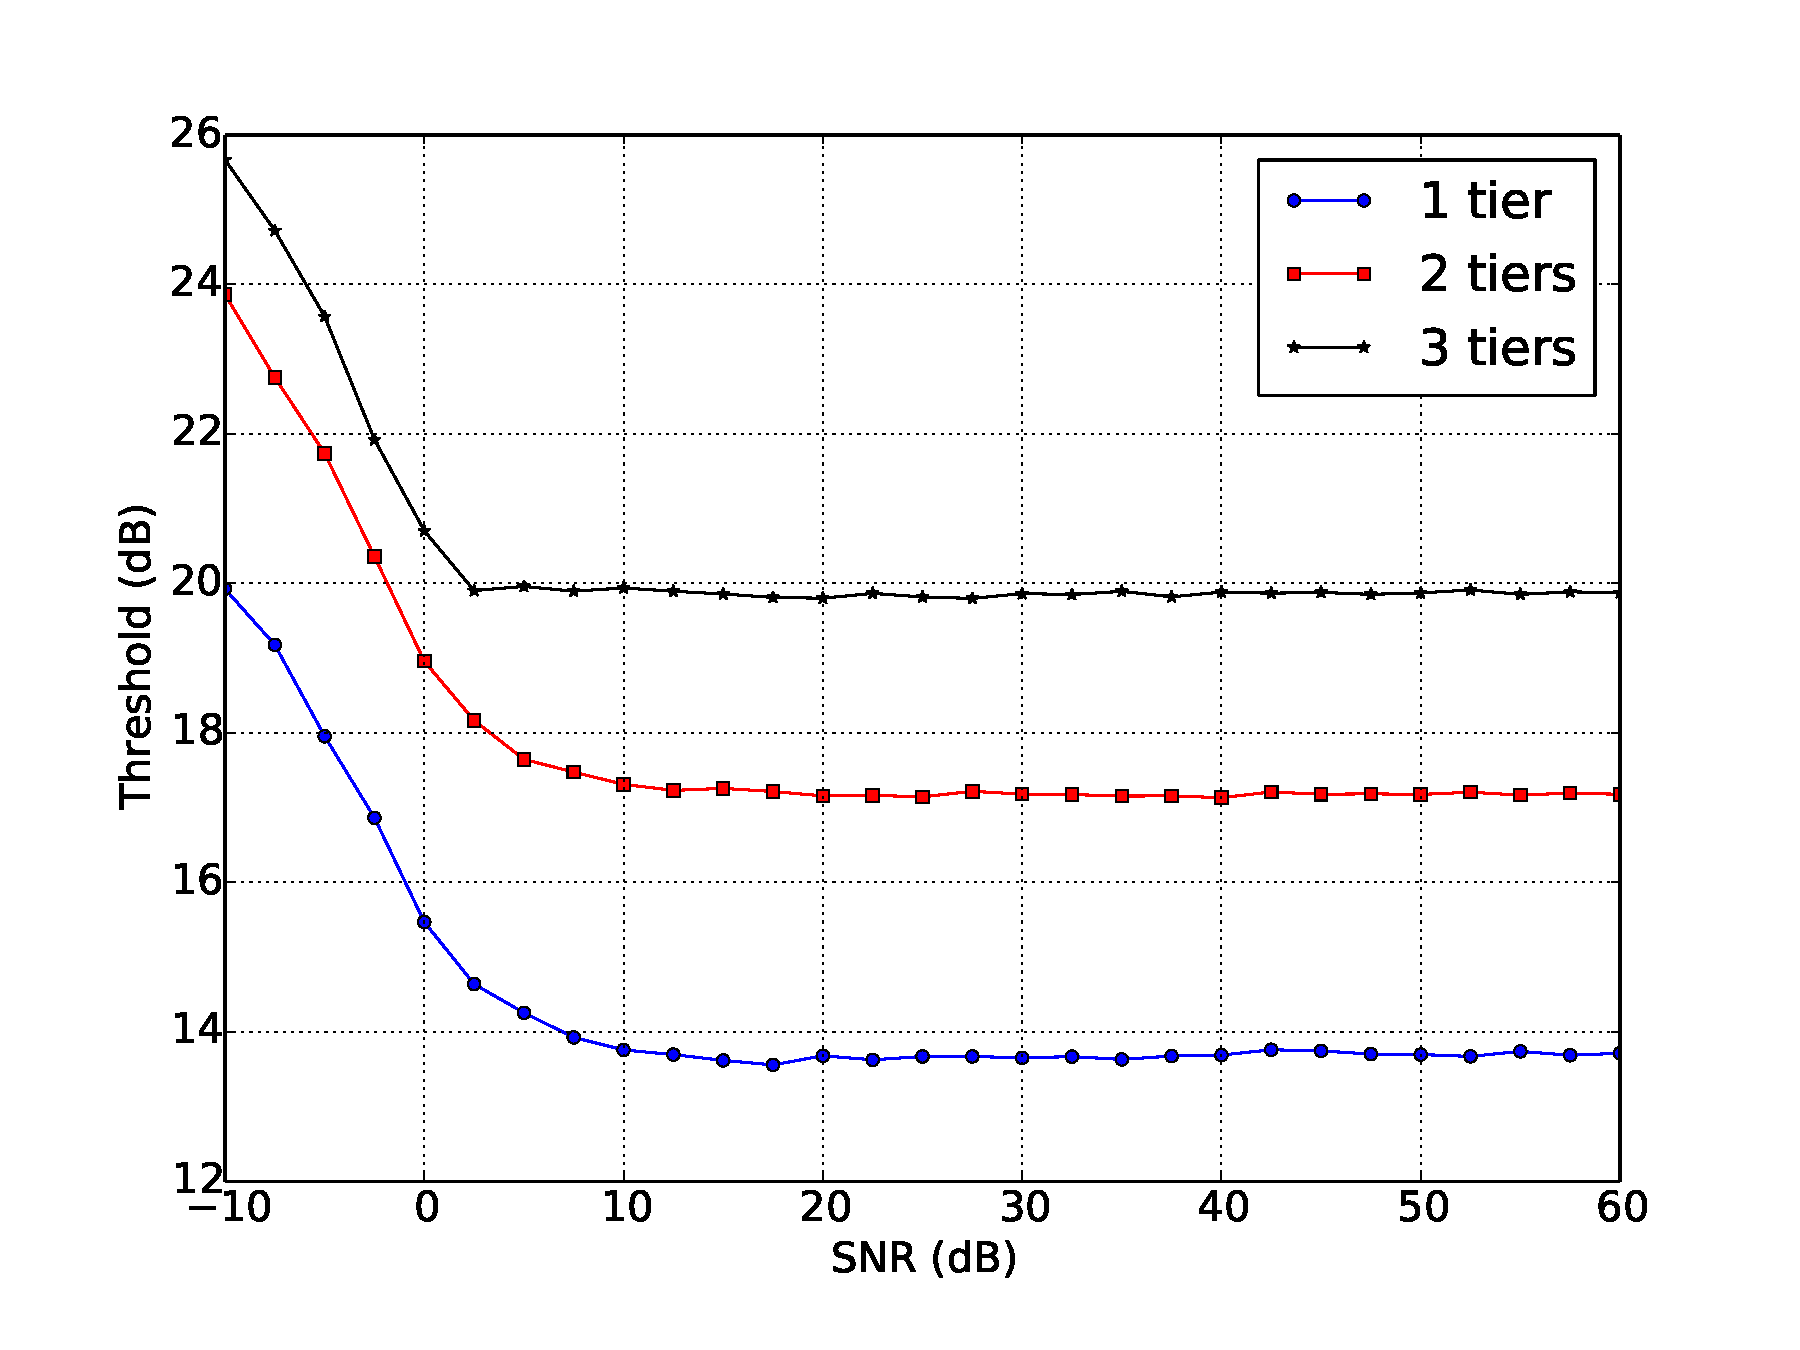
\includegraphics[width=0.75\columnwidth]{./21.appendices/figure/threshold_snr_tiers_02x02_c02_r1300}
    \caption{Threshold as a function of the \gls{snr}, for different cluster
    sizes, for $\gamma = 3.8$.}
	\label{fig:th_snr_tiers}
\end{figure}

\begin{figure}[t]
	\centering
	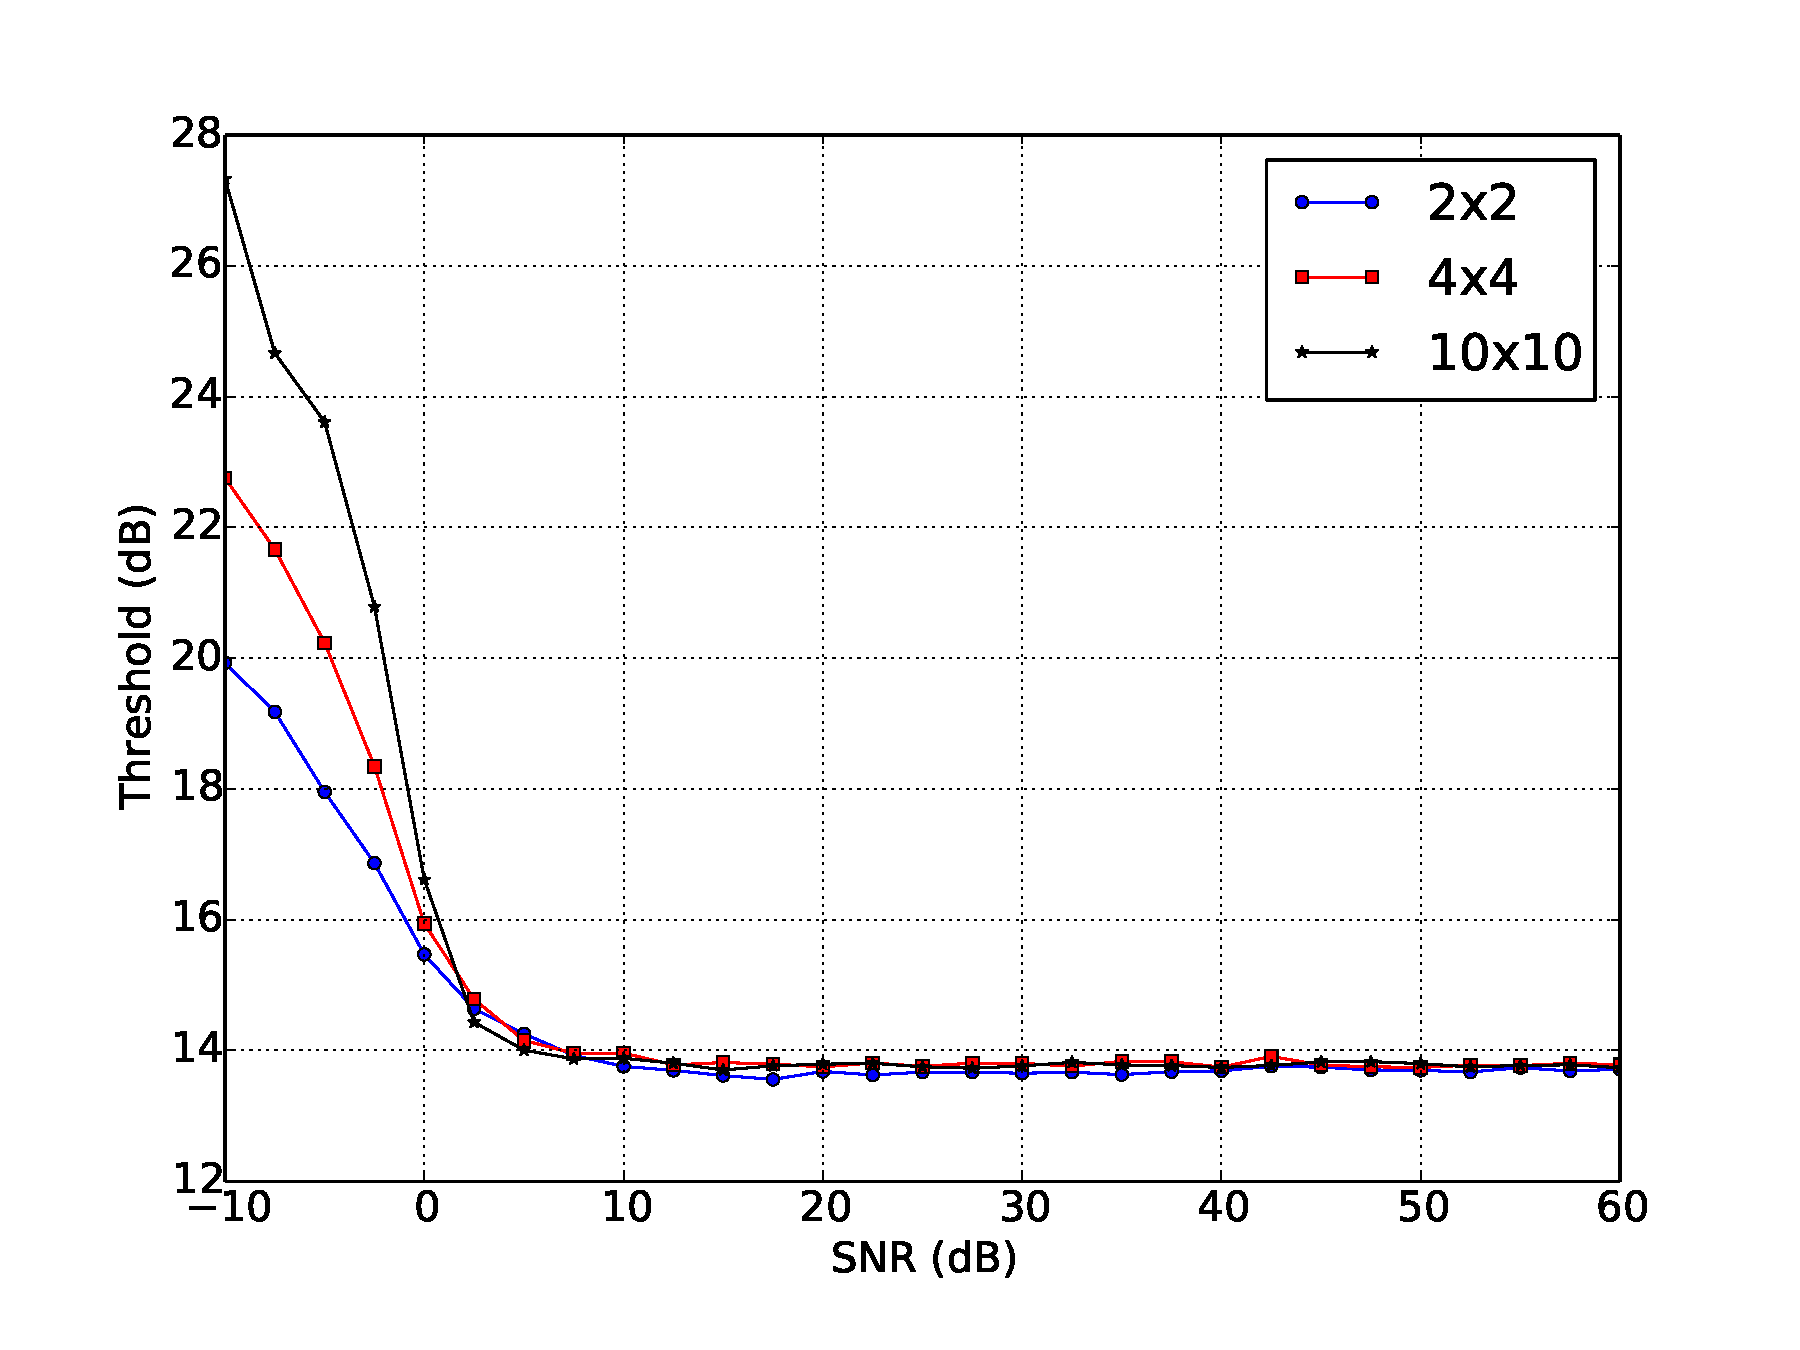
\includegraphics[width=0.75\columnwidth]{./21.appendices/figure/threshold_snr_anten_02x02_t02_i01_r1300}
    \caption{Threshold as a function of the \gls{snr}, for different \gls{mimo}
    configurations, for $\gamma = 3.8$.}
	\label{fig:th_snr_ant}
\end{figure}

